\documentclass{article}

% if you need to pass options to natbib, use, e.g.:
%     \PassOptionsToPackage{numbers, compress}{natbib}
% before loading neurips_2018

% ready for submission
\usepackage[nonatbib,preprint]{neurips_2019}
% \usepackage[nonatbib]{nips_2018}
\usepackage[numbers]{natbib}
% to compile a preprint version, e.g., for submission to arXiv, add add the
% [preprint] option:
%     \usepackage[preprint]{neurips_2018}

% to compile a camera-ready version, add the [final] option, e.g.:
    % \usepackage[preprint]{nips_2018}

% to avoid loading the natbib package, add option nonatbib:
    % \usepackage[nonatbib]{neurips_2018}

\usepackage[utf8]{inputenc} % allow utf-8 input
\usepackage[T1]{fontenc}    % use 8-bit T1 fonts
\usepackage{hyperref}       % hyperlinks
\usepackage{url}            % simple URL typesetting
\usepackage{booktabs}       % professional-quality tables
\usepackage{amsfonts}       % blackboard math symbols
\usepackage{nicefrac}       % compact symbols for 1/2, etc.
\usepackage{microtype}      % microtypography

\usepackage{algorithm}
\usepackage{algorithmic}
\usepackage{subcaption}
%\newcommand{\theHalgorithm}{\arabic{algorithm}}
\usepackage{amsmath}
\usepackage{amssymb}
\usepackage{amsthm}
\usepackage{mathtools}
\usepackage{natbib}
\usepackage{enumerate}
\usepackage{tikz}
\usepackage{graphicx}

\newtheorem{theorem}{Theorem}[section]
\newtheorem{proposition}{Proposition}[section]
\newtheorem{corollary}{Corollary}[theorem]
\newtheorem{conjecture}{Conjecture}[section]
\newtheorem{lemma}{Lemma}[section]
\newtheorem{corollaryp}{Corollary}[proposition]
\newtheorem{definition}{Definition}[section]
\newtheorem{assumption}{Assumption}[section]

\newcommand{\TODO}[1]{\textcolor{red}{TODO: #1}}
\newcommand{\citemissing}{\textcolor{red}{(cite?)}}

\DeclarePairedDelimiter\abs{\lvert}{\rvert}%
\DeclarePairedDelimiter\norm{\lVert}{\rVert}%
\DeclarePairedDelimiter\ceil{\lceil}{\rceil}
\DeclarePairedDelimiter\floor{\lfloor}{\rfloor}

\newcommand{\normt}[1]{\left\lVert#1\right\rVert_2}
\newcommand{\normm}[1]{\left\lVert#1\right\rVert}
\newcommand{\norminf}[1]{\left\lVert#1\right\rVert_\infty}
\newcommand{\normtt}[1]{\left\lVert#1\right\rVert^2_2}
\newcommand{\Ainv}{A^{-1}}
\newcommand{\half}{\frac{1}{2}}
\newcommand{\fourth}{\frac{1}{4}}
\newcommand{\xsum}{x^{sum}}
\newcommand{\ysum}{y^{sum}}
\newcommand{\vect}[1]{\overrightafrrow{\textbf{#1}}}
\newcommand{\phat}{\hat{p}}
\newcommand{\KL}[2]{D_{KL}(#1||#2)}
\newcommand{\TV}[2]{D_{TV}(#1||#2)}
\newcommand{\ind}[1]{1[#1]}
\newcommand{\pardiv}[1]{\frac{\partial}{\partial #1}}
\newcommand{\parHess}[1]{\frac{\partial^2}{\partial #1 ^2}}
\newcommand{\Xhat}{{\hat{X}}}
\newcommand{\xhat}{{\hat{x}}}
\newcommand{\Qhalf}{Q^{\frac{1}{2}}}
\newcommand{\Qneghalf}{Q^{-\frac{1}{2}}}
\newcommand{\defeq}{\mathrel{\stackrel{\makebox[0pt]{\mbox{\normalfont\tiny def}}}{=}}}

\newcommand{\lambdabar}{{\bar{\lambda}}}
\newcommand{\argmax}[1]{\underset{#1}{\mathrm{argmax}}}
\newcommand{\argmin}[1]{\underset{#1}{\mathrm{argmin}}}
\newcommand{\grad}[1]{\nabla{#1}}
\newcommand{\innerp}[2]{\langle{#1,#2}\rangle}
\newcommand{\Hess}[1]{\nabla^2{#1}}
\newcommand{\EXP}[1]{\text{exp}\{#1\}}

% RL
\newcommand{\Rmax}{R_{\mathrm{max}}}
\newcommand{\data}[1]{\bar{#1}}
\newcommand{\datapi}{{\bar{\pi}}}
\newcommand{\newpi}{\pi^\mathrm{new}}
\newcommand{\Kret}[2]{\eta^{#1//#2}_K}
\newcommand{\Khatret}[2]{\hat{\eta}^{#1//#2}_K}
\newcommand{\Kprobsa}[2]{p^{#1//#2, K}}
\newcommand{\epsmodel}{\epsilon_m}
\newcommand{\epspi}{\epsilon_\pi}

\newcommand{\Proj}{\Pi}
\newcommand{\Projmu}{\Pi_\mu}
\newcommand{\trans}{P}
\newcommand{\backup}{\mathcal{T}}
\newcommand{\Qclass}{\mathcal{Q}}
\newcommand{\ReplayBuffer}{\mathcal{B}}
\newcommand{\ltwonorm}{{\ell_2}}
\newcommand{\linfnorm}{{\ell_\infty}}

\newcommand{\UniformVec}{U[-1,1]^{32}}
\newcommand{\Tpi}{\backup^\pi}
\newcommand{\TPi}{\backup^\Pi}
\newcommand{\VPi}{V^\Pi}
\newcommand{\Vpi}{V^\pi}
\newcommand{\QPi}{Q^\Pi}
\newcommand{\Qpi}{Q^\pi}
\newcommand{\pidata}{\Pi} 
\newcommand{\pidatacdot}{\Pi(\cdot|s)}
\newcommand{\picdot}{\pi(\cdot|s)}
\newcommand{\dataset}{\mathcal{D}}
\newcommand{\expec}{\mathbb{E}}
\newcommand{\rhoinit}{{\rho_0}}
\newcommand{\Pieps}{{\Pi_\epsilon}}


\newcommand{\imperr}{\epsilon}
\newcommand{\projerr}{\delta}
\newcommand{\polerr}{\delta}
\newcommand{\valerr}{\zeta}
\newcommand{\greedy}{\mathcal{G}}
\newcommand{\greedyPi}{\mathcal{G}^\Pi}

\newcommand{\mmd}{\operatorname{MMD}}

\newcommand{\cmt}[1]{{\textcolor{red}{#1}}}
\newcommand{\cmtblue}[1]{{\textcolor{blue}{#1}}}
\newcommand{\aviral}[1]{\cmtblue{#1}}
\usepackage{wrapfig}

\title{Stabilizing Off-Policy Q-Learning via Bootstrapping Error Reduction}


\newcommand*\samethanks[1][\value{footnote}]{\footnotemark[#1]}
\newcommand*\samethanksnew[1][\value{footnote}]{\footnotemark[#1]}

\newcommand\blfootnote[1]{%
  \begingroup
  \renewcommand\thefootnote{}\footnote{#1}%
  \addtocounter{footnote}{-1}%
  \endgroup
}


\author{%s
    Aviral Kumar$^*$~~$^1$,~ Justin Fu$^*$ ~$^1$,~ George Tucker$^2$,~ Sergey Levine$^1$\\
    $^1$BAIR, UC Berkeley, $^2$Google Brain, ($^*$ Equal Contribution)\\
    \texttt{\{aviralk, justinfu\}@berkeley.edu}
}

\begin{document}
% \nipsfinalcopy is no longer used

\maketitle
%\vspace{-10pt}
%\begin{abstract}
%\vspace{-10pt}
%Off-policy reinforcement learning aims to leverage experience collected from prior policies for sample-efficient learning. However, in practice, commonly used off-policy methods are highly sensitive to the data distribution. As a step towards more robust off-policy algorithms, we study the setting where the off-policy experience is fixed and there is no further interaction with the environment. We analyze how distribution shift and approximation errors result in sources of error which can impact performance, and based on our analysis, we propose a practical algorithm, bootstrapping error accumulation reduction (BEAR) which prevents backing up from actions lying outside the support of the train distribution thereby reducing approximation errors. We demonstrate that BEAR is able to learn robustly from different off-policy distributions, including random and suboptimal demonstrations, on a range of continuous control tasks.
%\end{abstract}

\vspace{-40pt}
\section{Introduction}
\vspace{-10pt}
One of the primary drivers of the success of machine learning methods in open-world perception settings, such as computer vision~\cite{he2016resnet} and NLP~\cite{devlin2018bert}, has been the ability of high-capacity function approximators, such as deep neural networks, to learn generalizable models from large amounts of data. Reinforcement learning (RL) has proven comparatively difficult to scale to unstructured real-world settings because most RL algorithms require active data collection. Algorithms that can utilize such datasets effectively would not only make real-world RL more practical, but also would enable substantially better generalization by incorporating diverse prior experience.  

Off-policy reinforcement learning aims to leverage experience collected from prior policies for sample-efficient learning. However, in practice, commonly used methods are highly sensitive to the data distribution, and can fail even when the data is optimal (i.e. collected from an expert policy). We study off-policy RL with static datasets without any interaction with the environment.

Our primary contribution is an analysis of error accumulation in the bootstrapping process due to out-of-distribution inputs and a practical algorithm, \emph{bootstrapping error accumulation reduction} (BEAR) for addressing this error. We formalize and analyze the reasons for instability and poor performance when learning from off-policy data. We then propose BEAR algorithm to control bootstrapping error in practice, which uses the notion of \emph{support-set constraints} to prevent error accumulation due to out-of-distribution inputs during bootstrapping. We demonstrate that BEAR is able to learn robustly from different off-policy distributions, including random and suboptimal demonstrations, on a range of continuous control tasks.

\vspace{-11pt}
\section{Error Propagation from Out-of-Distribution Inputs}
\vspace{-10pt}
\begin{wrapfigure}{r}{0.5\textwidth}
\vspace{-10pt}
\begin{center}
\vspace{-0.1in}
    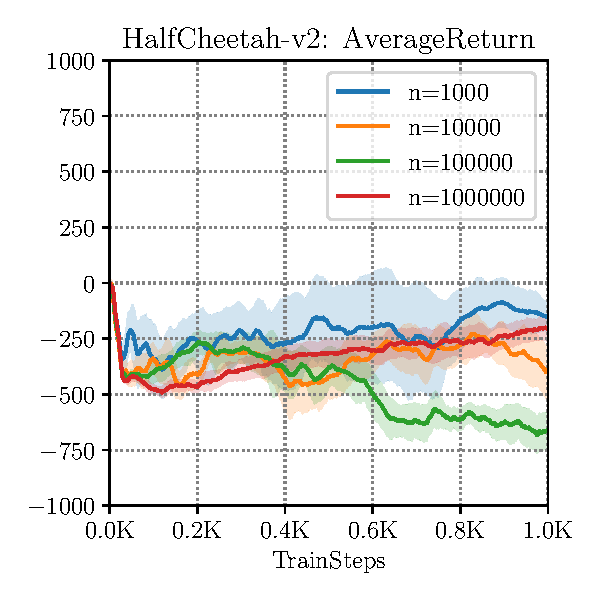
\includegraphics[width=0.48\linewidth]{images/cheetah_divergence.pdf}
    ~
    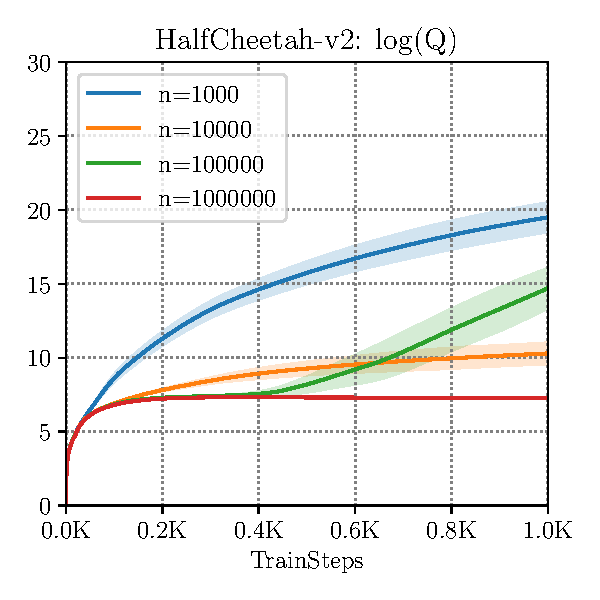
\includegraphics[width=0.48\linewidth]{images/cheetah_divergence_q_val.pdf}
  \end{center}
 \vspace{-10pt}
\caption{ \footnotesize Performance of SAC on HalfCheetah-v2 (return (left) and $\log$ Q-values (right)) with off-policy expert data w.r.t. number of training samples ($n$).} 
 \vspace{-15pt}
 \label{fig:divergence}
\end{wrapfigure}
Q-learning methods often fail to learn on static, off-policy data, as shown in Figure \ref{fig:divergence}. Note the large discrepancy between returns (which are negative) and $\log$ Q-values (which have large positive values), which is not solved with additional samples. Errors in the Bellman backup can easily arise when Q-values are queried on out-of-distribution inputs. For example, in the computation of the value function, $V(s) = \max_a Q(s,a)$, the max operator can easily query Q on actions not seen in the data, resulting in potentially uncontrolled errors.

Formally, let $\valerr_k(s, a) = |Q_k(s,a) - Q^*(s,a)|$ denote the total error at iteration $k$ of Q-learning, and let $\projerr_k(s, a) = |Q_k(s,a) - \backup Q_{k-1}(s,a)|$ denote the current Bellman error. Then, we have \mbox{$\valerr_k(s, a) \le \projerr_k(s,a) + \gamma \max_{a'} \expec_{s'}[\valerr_{k-1}(s',a')]$}. In other words, errors from $(s', a')$ are discounted, then accumulated with new errors $\projerr_k(s, a)$ from the current iteration. We expect $\projerr_k(s,a)$ to be high on out-of-distribution (OOD) states and actions, as errors at these state-actions are never directly minimized while training.



\vspace{-10pt}
\section{Error Reduction through Constrained Backups}
\vspace{-10pt}

Our method for error reduction involves constraining the Bellman backup operator to in-distribution inputs, in order to reduce the propagation of errors from uncontrolled, out-of-distribution values. We define the constrained backup as follows:
\begin{definition}[Distribution-constrained operators]
Given a set of policies $\Pi$
, the distribution-constrained backup operator is defined as:
\begin{align*}
\TPi Q(s, a) \defeq \expec \big[ R(s, a) + \gamma \max_{\pi \in \Pi} \expec_{\trans(s' | s, a)}\left[V(s') \right] \big]
\ \ \ \ \ \ \ \ \ \ \ \ 
V(s) \defeq \max_{\pi \in \Pi} \expec_{\pi}[Q(s, a)]\ \ .
\end{align*}
\end{definition}
Using such a backup operator, we can bound the error resulting from running dynamic programming as follows:
\begin{theorem}
\label{thm:avi_bound}
Suppose we run approximate distribution-constrained value iteration with a set constrained backup $\TPi$. Assume that $\delta(s,a) \ge \max_k |Q_k(s,a) - \TPi Q_{k-1}(s,a)|$ bounds the Bellman error. Then,
\[\lim_{k \to \infty} \expec_{\rhoinit}[|V^{\pi_k}(s) - V^*(s)|] \le
\frac{\gamma}{(1-\gamma)^2}\left[ C(\Pi)\expec_\mu[\max_{\pi \in \Pi} \expec_{\pi}[\projerr(s,a)]] + \frac{1-\gamma}{\gamma}\alpha(\Pi) \right]
\]
\end{theorem}

Where $C(\Pi)$ is a concentrability coefficient (defined in ~\citep{munos2005erroravi}), measuring how off-policy the data is, and $\alpha(\Pi)= \max_{s,a} |\TPi Q^*(s, a) - \backup Q^*(s, a)|.$ is a suboptimality coefficient, measuring how restrictive $\Pi$ is in terms of the optimal policy.
The intuition is that the more we restrict the policy to the data, the lower $C(\Pi)$ becomes, but the higher $\alpha(\Pi)$ becomes. Thus, the choice of $\Pi$ becomes a tradeoff between suboptimality and degree of ``off-policy-ness''.

We use support sets to construct $\Pi$. We are interested in the case where $\Pi = \{ \pi ~|~ \pi( a | s) = 0 \text{ whenever } \beta( a | s) < \epsilon \}$, where $\beta$ is the behavior policy (i.e., $\Pi$ is the set of policies that have support in the probable regions of the behavior policy). Defining $\Pi$ in this way allows us to bound the concentrability coefficient. 

\section{Method and Experiments}
We instantiate our BEAR (also called BEAR-QL) algorithm on deep RL domains built on the framework of TD3~\cite{fujimoto18addressing} that uses constrained backups to reduce accumulation of bootstrapping error. Our algorithm has two main components. We use ensembles of Q-functions to provide a conservative estimate of the Q-function for policy improvement, and design a constraint which will be used for searching over the set of policies $\Pi$, which share the same support as the behaviour policy. Both of these components will appear as modifications of only the policy improvement step in common actor-critic style algorithms. Mathematically, thw new policy improvement step is given by: ($\hat{Q}_k$ is the k-th member of the ensemble of Q functions, and $\operatorname{MMD}(\cdot, \cdot)$ is the maximum mean discrepancy~\cite{gretton2012kernel} distance (which can provide support matching behaviour under some assumptions)   
\vspace{-5pt}
\begin{multline}
    \label{eqn:policy_update}
   \pi_\phi(s) := \max_{\pi \in \Delta_{|S|}} \expec_{a \sim \pi(\cdot|s)} [\hat{Q}_{k}(s, a)] - \lambda \sqrt{ \operatorname{var_k}\expec_{a \sim \pi(\cdot |s) }[\hat{Q}_k(s, a)]}\\
   \text{~~s.t.~~} \mathbb{E}_{s \sim \mathcal{D}} [\operatorname{MMD}(\mathcal{D}(s), \pi(\cdot|s))] \leq \varepsilon
\end{multline}

We evaluate our BEAR-QL algorithm in three settings: when the dataset $\dataset$ is generated by \textbf{(1)} a completely random behaviour policy, \textbf{(2)} a partially trained, medium scoring policy, and \textbf{(3)} an optimal policy. 
Example results for the HalfCheetah domain are shown in Fig.~\ref{fig:mediocre}. We find that BEAR achieves consistent results across datasets, outperforming BCQ~\cite{fujimoto2018off}, naive RL and behaviour cloning (BC). The same trend holds true across multiple MuJoCo tasks (Ant-v2, Hopper-v2 and Walker2d-v2).

% \begin{figure*}[b!]
\begin{wrapfigure}{r}{0.99\textwidth}
    \centering
    \vspace{-0.05in}
    \begin{subfigure}[t]{0.23\textwidth}
        \centering
        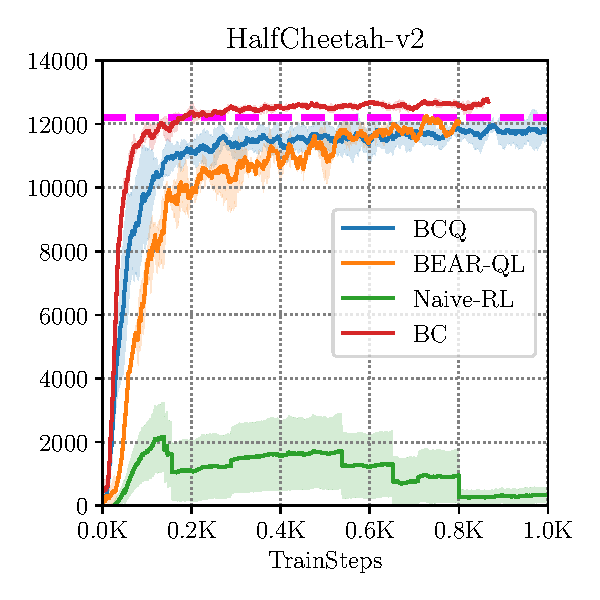
\includegraphics[width=0.99\linewidth]{images/cheetah_optimal_final.pdf}
    \end{subfigure}
    \begin{subfigure}[t]{0.23\textwidth}
        \centering
        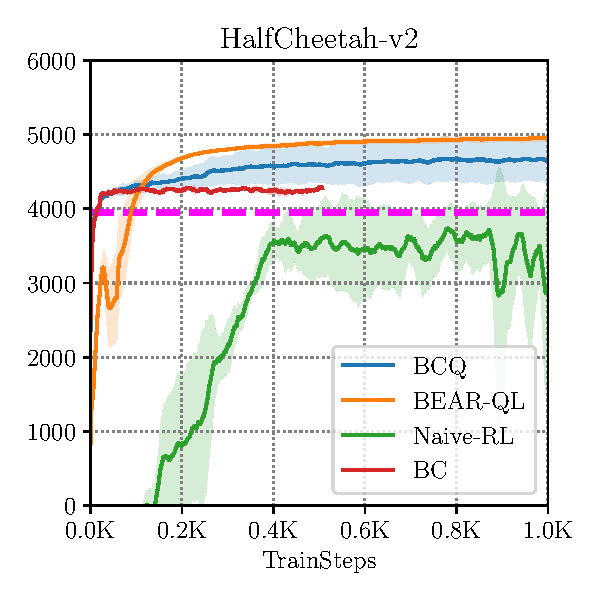
\includegraphics[width=0.99\linewidth]{images/cheetah_mediocre.pdf}
        % \caption{}
    \end{subfigure}
    \begin{subfigure}[t]{0.23\textwidth}
        \centering
        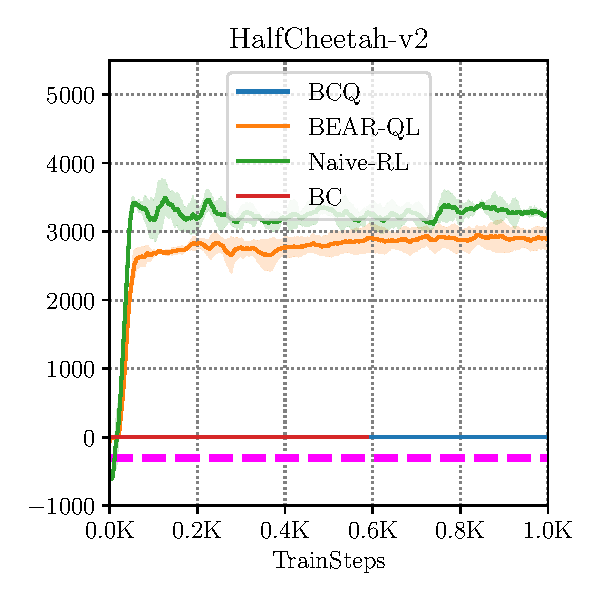
\includegraphics[width=0.99\linewidth]{images/cheetah_random_final.pdf}
        % \caption{}
    \end{subfigure}
    \caption{ \footnotesize Performance of BEAR-QL, BCQ, Na\"ive RL and BC on the HalfCheetah domain. (\textbf{Left}: Expert data, \textbf{Middle}: Medium-quality data, \textbf{Right}: Random data) BEAR performs consistently across all types of data, and outperforms BCQ, Na\"ive RL and BC. Average return over the training data is indicated by the magenta line.}
    \label{fig:mediocre}
    \vspace{-0.1in}
\end{wrapfigure}

\clearpage
\bibliography{example_paper}
\bibliographystyle{plainnat}

\end{document}
